\documentclass[a4paper]{article}

\usepackage{inputenc}
\usepackage[british,UKenglish]{babel}
\usepackage{amsmath}
%\usepackage{titlesec}
\usepackage{color}
\usepackage{graphicx}
\usepackage{fancyref}
\usepackage{hyperref}
\usepackage{float}
\usepackage{scrextend}
\usepackage{setspace}
\usepackage{xargs}
\usepackage{multicol}
\usepackage{nameref}

\usepackage{sectsty}
\usepackage{multicol}
\usepackage{multirow}
\usepackage[procnames]{listings}
\usepackage{appendix}

\newcommand\tab[1][1cm]{\hspace*{#1}}
\hypersetup{colorlinks=true, linkcolor=black}
\interfootnotelinepenalty=10000

\newcommand{\cleancode}[1]{\begin{addmargin}[3em]{3em}\texttt{\textcolor{cleanOrange}{#1}}\end{addmargin}}
\newcommand{\cleanstyle}[1]{\text{\textcolor{cleanOrange}{\texttt{#1}}}}


\usepackage[colorinlistoftodos,prependcaption,textsize=footnotesize]{todonotes}
\newcommandx{\commred}[2][1=]{\textcolor{Red}
{\todo[linecolor=red,backgroundcolor=red!25,bordercolor=red,#1]{#2}}}
\newcommandx{\commblue}[2][1=]{\textcolor{Blue}
{\todo[linecolor=blue,backgroundcolor=blue!25,bordercolor=blue,#1]{#2}}}
\newcommandx{\commgreen}[2][1=]{\textcolor{OliveGreen}{\todo[linecolor=OliveGreen,backgroundcolor=OliveGreen!25,bordercolor=OliveGreen,#1]{#2}}}
\newcommandx{\commpurp}[2][1=]{\textcolor{Plum}{\todo[linecolor=Plum,backgroundcolor=Plum!25,bordercolor=Plum,#1]{#2}}}

\def\code#1{{\tt #1}}

\def\note#1{\noindent{\bf [Note: #1]}}

\makeatletter
%% The "\@seccntformat" command is an auxiliary command
%% (see pp. 26f. of 'The LaTeX Companion,' 2nd. ed.)
\def\@seccntformat#1{\@ifundefined{#1@cntformat}%
   {\csname the#1\endcsname\quad}  % default
   {\csname #1@cntformat\endcsname}% enable individual control
}
\let\oldappendix\appendix %% save current definition of \appendix
\renewcommand\appendix{%
    \oldappendix
    \newcommand{\section@cntformat}{\appendixname~\thesection\quad}
}
\makeatother


% "define" Scala
\usepackage[T1]{fontenc}  
\usepackage[scaled=0.82]{beramono}  
\usepackage{microtype} 

\sbox0{\small\ttfamily A}
\edef\mybasewidth{\the\wd0 }

\lstdefinelanguage{scala}{
  morekeywords={abstract,case,catch,class,def,%
    do,else,extends,false,final,finally,%
    for,if,implicit,import,match,mixin,%
    new,null,object,override,package,%
    private,protected,requires,return,sealed,%
    super,this,throw,trait,true,try,%
    type,val,var,while,with,yield},
  sensitive=true,
  morecomment=[l]{//},
  morecomment=[n]{/*}{*/},
  morestring=[b]",
  morestring=[b]',
  morestring=[b]"""
}

\usepackage{color}
\definecolor{dkgreen}{rgb}{0,0.6,0}
\definecolor{gray}{rgb}{0.5,0.5,0.5}
\definecolor{mauve}{rgb}{0.58,0,0.82}

% Default settings for code listings
\lstset{frame=tb,
  language=scala,
  aboveskip=3mm,
  belowskip=3mm,
  showstringspaces=false,
  columns=fixed, % basewidth=\mybasewidth,
  basicstyle={\small\ttfamily},
  numbers=none,
  numberstyle=\footnotesize\color{gray},
  % identifierstyle=\color{red},
  keywordstyle=\color{blue},
  commentstyle=\color{dkgreen},
  stringstyle=\color{mauve},
  frame=single,
  breaklines=true,
  breakatwhitespace=true,
  procnamekeys={def, val, var, class, trait, object, extends},
  procnamestyle=\ttfamily\color{red},
  tabsize=2
}

\lstnewenvironment{scala}[1][]
{\lstset{language=scala,#1}}
{}
\lstnewenvironment{cpp}[1][]
{\lstset{language=C++,#1}}
{}
\lstnewenvironment{bash}[1][]
{\lstset{language=bash,#1}}
{}
\lstnewenvironment{verilog}[1][]
{\lstset{language=verilog,#1}}
{}



%代码段设置
\lstset{numbers=left,
basicstyle=\tiny,
numberstyle=\tiny,
keywordstyle=\color{blue!70},
commentstyle=\color{red!50!green!50!blue!50},
frame=single, rulesepcolor=\color{red!20!green!20!blue!20},
escapeinside=``
}

\graphicspath{ {images/} }
\usepackage{ctex}
\usepackage{graphicx}
\usepackage{color,framed}%文本框
\usepackage{listings}
\usepackage{caption}
\usepackage{amssymb}
\usepackage{enumerate}
\usepackage{xcolor}
\usepackage{bm} 
\usepackage{lastpage}%获得总页数
\usepackage{fancyhdr}
\usepackage{tabularx}  
\usepackage{geometry}
\usepackage{graphics}
\usepackage{subfigure}
\usepackage{float}
\usepackage{pdfpages}
\usepackage{pgfplots}
\pgfplotsset{width=10cm,compat=1.9}
\usepackage{multirow}
\usepackage{footnote}
\usepackage{booktabs}
\usepackage{url}

%-----------------------伪代码------------------
\usepackage{algorithm}  
\usepackage{algorithmicx}  
\usepackage{algpseudocode}  
\floatname{algorithm}{Algorithm}  
\renewcommand{\algorithmicrequire}{\textbf{Input:}}  
\renewcommand{\algorithmicensure}{\textbf{Output:}} 
\usepackage{lipsum}  
\makeatletter
\newenvironment{breakablealgorithm}
  {% \begin{breakablealgorithm}
  \begin{center}
     \refstepcounter{algorithm}% New algorithm
     \hrule height.8pt depth0pt \kern2pt% \@fs@pre for \@fs@ruled
     \renewcommand{\caption}[2][\relax]{% Make a new \caption
      {\raggedright\textbf{\ALG@name~\thealgorithm} ##2\par}%
      \ifx\relax##1\relax % #1 is \relax
         \addcontentsline{loa}{algorithm}{\protect\numberline{\thealgorithm}##2}%
      \else % #1 is not \relax
         \addcontentsline{loa}{algorithm}{\protect\numberline{\thealgorithm}##1}%
      \fi
      \kern2pt\hrule\kern2pt
     }
  }{% \end{breakablealgorithm}
     \kern2pt\hrule\relax% \@fs@post for \@fs@ruled
  \end{center}
  }
\makeatother
%------------------------代码-------------------
\usepackage{xcolor} 
\usepackage{listings} 
\lstset{ 
breaklines,%自动换行
basicstyle=\small\ttfamily,
escapeinside=``,
keywordstyle=\color{blue!70}\bfseries,
commentstyle=\color{red!50!green!50!blue!50},
stringstyle=\color{red}\ttfamily,
extendedchars=false,
linewidth=\textwidth,
numbers=left,
numberstyle=\tiny\color{blue!50},
frame=trbl,
rulesepcolor=\color{red!20!green!20!blue!20},
showstringspaces=false,
tabsize=4,
captionpos=b
}

% 定义更多语言的关键词高亮
\lstdefinelanguage{Python}{
    keywords={def,class,if,else,elif,for,while,try,except,import,from,as,return,break,continue,pass,with,yield,lambda,global,nonlocal,True,False,None},
    keywordstyle=\color{blue!70}\bfseries,
    sensitive=true,
    comment=[l]{\#},
    string=[s]{'}{'},
    morestring=[s]{"}{"}
}

%-------------------------页面边距--------------
\geometry{a4paper,left=2.3cm,right=2.3cm,top=2.7cm,bottom=2.7cm}
%-------------------------页眉页脚--------------
\usepackage{fancyhdr}
\pagestyle{fancy}
\lhead{\kaishu \leftmark}
% \chead{}
\rhead{\kaishu 并行程序设计实验报告}%加粗\bfseries 
\lfoot{}
\cfoot{\thepage\ of \pageref{LastPage}}%当前页 of 总页数
\rfoot{}
\renewcommand{\headrulewidth}{0.1pt}  
\renewcommand{\footrulewidth}{0pt}%去掉横线
\newcommand{\HRule}{\rule{\linewidth}{0.5mm}}%标题横线
\newcommand{\HRulegrossa}{\rule{\linewidth}{1.2mm}}
\setlength{\textfloatsep}{10mm}%设置图片的前后间距
%--------------------文档内容--------------------

\begin{document}
\renewcommand{\contentsname}{目\ 录}
\renewcommand{\appendixname}{附录}
\renewcommand{\appendixpagename}{附录}
\renewcommand{\refname}{参考文献} 
\renewcommand{\figurename}{图}
\renewcommand{\tablename}{表}
\renewcommand{\today}{\number\year 年 \number\month 月 \number\day 日}

%-------------------------封面----------------
\begin{titlepage}
    \begin{center}
    
\includegraphics[width=0.8\textwidth]{fig/NKU.png}\\[1cm]
    \vspace{20mm}
		\textbf{\huge\textbf{\kaishu{计算机学院}}}\\[0.5cm]
		\textbf{\huge{\kaishu{并行程序设计报告}}}\\[2.3cm]
		\textbf{\Huge\textbf{\kaishu{NTT MPI优化实验报告}}}

		\vspace{\fill}
    
    % \textbf{\Large \textbf{并行程序设计期末实验报告}}\\[0.8cm]
    % \HRule \\[0.9cm]
    % \HRule \\[2.0cm]
    \centering
    \textsc{\LARGE \kaishu{姓名\ :\ 廖望}}\\[0.5cm]
    \textsc{\LARGE \kaishu{学号\ :\ 2210556}}\\[0.5cm]
    \textsc{\LARGE \kaishu{专业\ :\ 计算机科学与技术}}\\[0.5cm]
    
    \vfill
    {\Large \today}
    \end{center}
\end{titlepage}

% 摘要
\begin{abstract}
    \textbf{摘要: }本报告深入探讨并评估了基于消息传递接口(MPI)的并行数论变换(NTT)算法的实现与性能。NTT作为快速傅里叶变换(FFT)在有限域上的推广,在密码学及高效多项式乘法等领域具有关键应用。本研究通过引入Barrett模约简等优化技术,旨在显著提升大规模多项式乘法的计算效率。实验在WSL Ubuntu 24.04环境下,利用OpenMPI对不同模数、数据规模(1000、10000、100000)以及进程数(1、2、4、8)配置下的并行NTT算法进行了系统性的性能测试。实验结果表明,该并行NTT算法在特定配置下展现出显著的加速效果,最高加速比达2.22倍。尤其在中大规模数据处理(10000和100000)时,2进程配置普遍实现了计算性能与通信开销的最佳平衡。本研究不仅证实了MPI并行NTT在提升计算效率方面的潜力,还对通信开销、负载不均衡及模数特性对并行性能的影响进行了详细分析,为高性能计算环境中数论变换的进一步优化提供了有益的经验与指导。完整的源代码和实验数据已开源至:\url{https://github.com/aokimi0/parallel-programming}。

    \vspace{1em}
    \textbf{关键词: }并行计算; MPI; 数论变换; NTT; Barrett模约简; 性能优化
\end{abstract}

\renewcommand {\thefigure}{\thesection{}.\arabic{figure}}%图片按章标号
\renewcommand{\figurename}{图}
\renewcommand{\contentsname}{目录}  
\cfoot{\thepage\ of \pageref{LastPage}}%当前页 of 总页数


% 生成目录
\clearpage
\tableofcontents
\newpage

%--------------------------Title--------------------------------
\section{引言}

数论变换(Number Theoretic Transform, NTT)是快速傅里叶变换(Fast Fourier Transform, FFT)在有限域上的扩展形式,在现代密码学、高效多项式乘法以及信号处理等领域中展现出重要的应用价值。与传统的FFT依赖复数单位根不同,NTT利用模意义下的原根进行运算,从而避免了浮点数计算带来的精度问题,在同态加密等对精度要求极为严苛的场景中尤其具有显著优势。

本实验旨在实现一个高效的MPI(Message Passing Interface)并行NTT算法,并对其性能进行深入的实证分析。在前期多线程实现经验的基础上,本研究进一步集成了Barrett模约简等关键优化技术,以期大幅提升大规模多项式乘法的计算效率。通过在不同MPI进程数量和多种数据规模下进行全面的性能测试,本报告旨在系统评估所实现的并行算法的加速效果、并行效率及可扩展性,为未来在大规模并行计算环境中优化数论变换提供有价值的参考依据。

\section{算法原理}

\subsection{数论变换基础}

数论变换(NTT)作为FFT的模域对应,其核心基于特定模数$p$下的原根性质。设$p$为一个质数,且$n$为2的幂次并满足$n|(p-1)$。在此前提下,我们定义$\omega_n = g^{(p-1)/n}$为$n$阶本原单位根,其中$g$是模$p$的原根。基于此,数论变换(NTT)被定义为:

$$Y_k = \sum_{j=0}^{n-1} X_j \omega_n^{jk} \bmod p$$

其逆变换为:
$$X_j = n^{-1} \sum_{k=0}^{n-1} Y_k \omega_n^{-jk} \bmod p$$

上述公式体系构成了NTT的核心数学基础,其关键优势在于能够将多项式乘法转化为复杂度更低的点值乘法,从而有效避免了传统卷积算法的高计算开销。

\subsection{Barrett模约简}

Barrett模约简是一种高效的模运算优化技术,尤其适用于模数固定且需进行大量模运算的场景。对于给定的模数$q$,该方法通过预先计算一个常数$r = \lfloor 2^k/q \rfloor$(其中$k$通常设定为机器字长,本实验中取64位),将计算成本较高的除法运算近似转换为一系列效率更高的乘法和位移操作。其核心计算过程可以表示为:

$$x \bmod q \approx x - \lfloor xr/2^k \rfloor \cdot q$$

这种优化策略能够显著降低模运算的平均执行时间,原因是它避免了浮点除法,转而利用整数乘法和位移指令,这些操作在现代处理器架构上通常具有更高的执行效率,并特别适用于SIMD(单指令多数据)并行优化。

\subsection{MPI并行策略}

本实验的MPI并行策略采用了主从计算模式,结合多项式乘法的并行化来实现整体性能提升:

\textbf{1. 主从NTT计算}:在该策略中,NTT变换本身由主进程串行执行,利用优化的Barrett模约简技术确保计算效率。计算完成后,主进程通过\texttt{MPI\_Bcast}将变换结果广播给所有其他进程。这种方法避免了复杂的蝶形运算同步问题,确保了算法的稳定性和可靠性。

\textbf{2. 点值乘法并行}:真正的并行化体现在多项式乘法的点值运算阶段。在两个多项式完成NTT变换后,每个进程负责计算分配给它的点值乘法子集。具体而言,每个进程处理\texttt{elements\_per\_proc}个元素的乘法运算,随后通过\texttt{MPI\_Allgather}集体通信操作汇聚所有进程的计算结果,形成完整的点值乘积向量。这种策略在多项式乘法这一计算密集型操作中实现了有效的负载分担。

\section{实现细节}

本节详细阐述了MPI并行NTT算法在C++中的具体实现,包括关键数据结构的设计和并行策略的编程实现。

\subsection{核心数据结构}

为了实现高效的模数运算,本实验引入了Barrett模约简技术。其核心功能被封装在\texttt{BarrettReduction}结构体中,其定义如下所示:

\begin{lstlisting}[title=Barrett规约结构,frame=trbl,language={C++}]
struct BarrettReduction {
    ll mod;
    __int128 r;
    int k;
    
    BarrettReduction(ll m) : mod(m) {
        k = 64;
        r = ((__int128)1 << k) / mod;
    }
    
    ll reduce(__int128 x) const {
        __int128 q = (x * r) >> k;
        __int128 result = x - q * mod;
        if (result >= mod) result -= mod;
        if (result < 0) result += mod;
        return (ll)result;
    }
    
    ll multiply(ll a, ll b) const {
        return reduce((__int128)a * b);
    }
};
\end{lstlisting}
此结构体通过预计算一个关键常数\texttt{r},从而实现了快速的模乘和模约简操作。该实现采用128位整数确保中间计算的精度,并包含了对负数结果的处理逻辑,有效规避了传统除法运算所带来的性能瓶颈,对于显著提升NTT算法的整体计算效率具有至关重要的作用。

\subsection{MPI蝶形运算并行}

MPI并行NTT的实现采用了主从计算模式。以下C++代码片段展示了\texttt{ntt\_mpi\_butterfly}函数的实际实现:

\begin{lstlisting}[title=MPI并行NTT实现,frame=trbl,language={C++}]
void ntt_mpi_butterfly(std::vector<ll>& a, bool invert, ll mod, ll root, 
                      int rank, int size) {
    if (rank == 0) {
        ntt_sequential_barrett(a, invert, mod, root);
    }
    MPI_Bcast(&a[0], a.size(), MPI_LONG_LONG, 0, MPI_COMM_WORLD);
}
\end{lstlisting}
该函数采用了简化的并行策略:主进程(rank 0)负责执行完整的串行Barrett优化NTT计算,计算完成后通过\texttt{MPI\_Bcast}将结果广播给所有其他进程。这种实现策略虽然在算法层面并未实现真正的并行蝶形运算,但通过将NTT计算与其他并行任务(如多项式点值乘法)相结合,仍能在整体应用中获得性能收益。该策略的优势在于实现简单、通信开销相对固定,避免了复杂并行蝶形运算中可能出现的同步开销和负载不均衡问题。

\section{实验结果与分析}

\subsection{计时方法}

为确保实验结果的准确性与可靠性,本实验严格遵循MPI标准,采用\texttt{MPI\_Wtime()}函数进行计算时间的精确测量。为有效消除单次测量的偶然误差并更准确地反映算法的平均性能,每个测试配置均重复运行10次,最终报告的结果为这10次运行时间的平均值。这种多次测量取均值的实践,是科学实验中普遍采用的方法,旨在提高数据的统计显著性。

\subsection{大规模性能测试}

本实验在WSL Ubuntu 24.04环境下进行,并以OpenMPI作为并行计算的实现框架。我们对MPI并行NTT算法的性能进行了全面的评估,测试涵盖3种不同的模数以及3种大规模数据尺寸下的表现。具体而言,测试所用的多项式系数规模分别为1000、10000和100000。同时,我们考察了在1、2、4、8个不同进程数配置下算法的实际运行效果。

\begin{figure}[H]
    \centering
    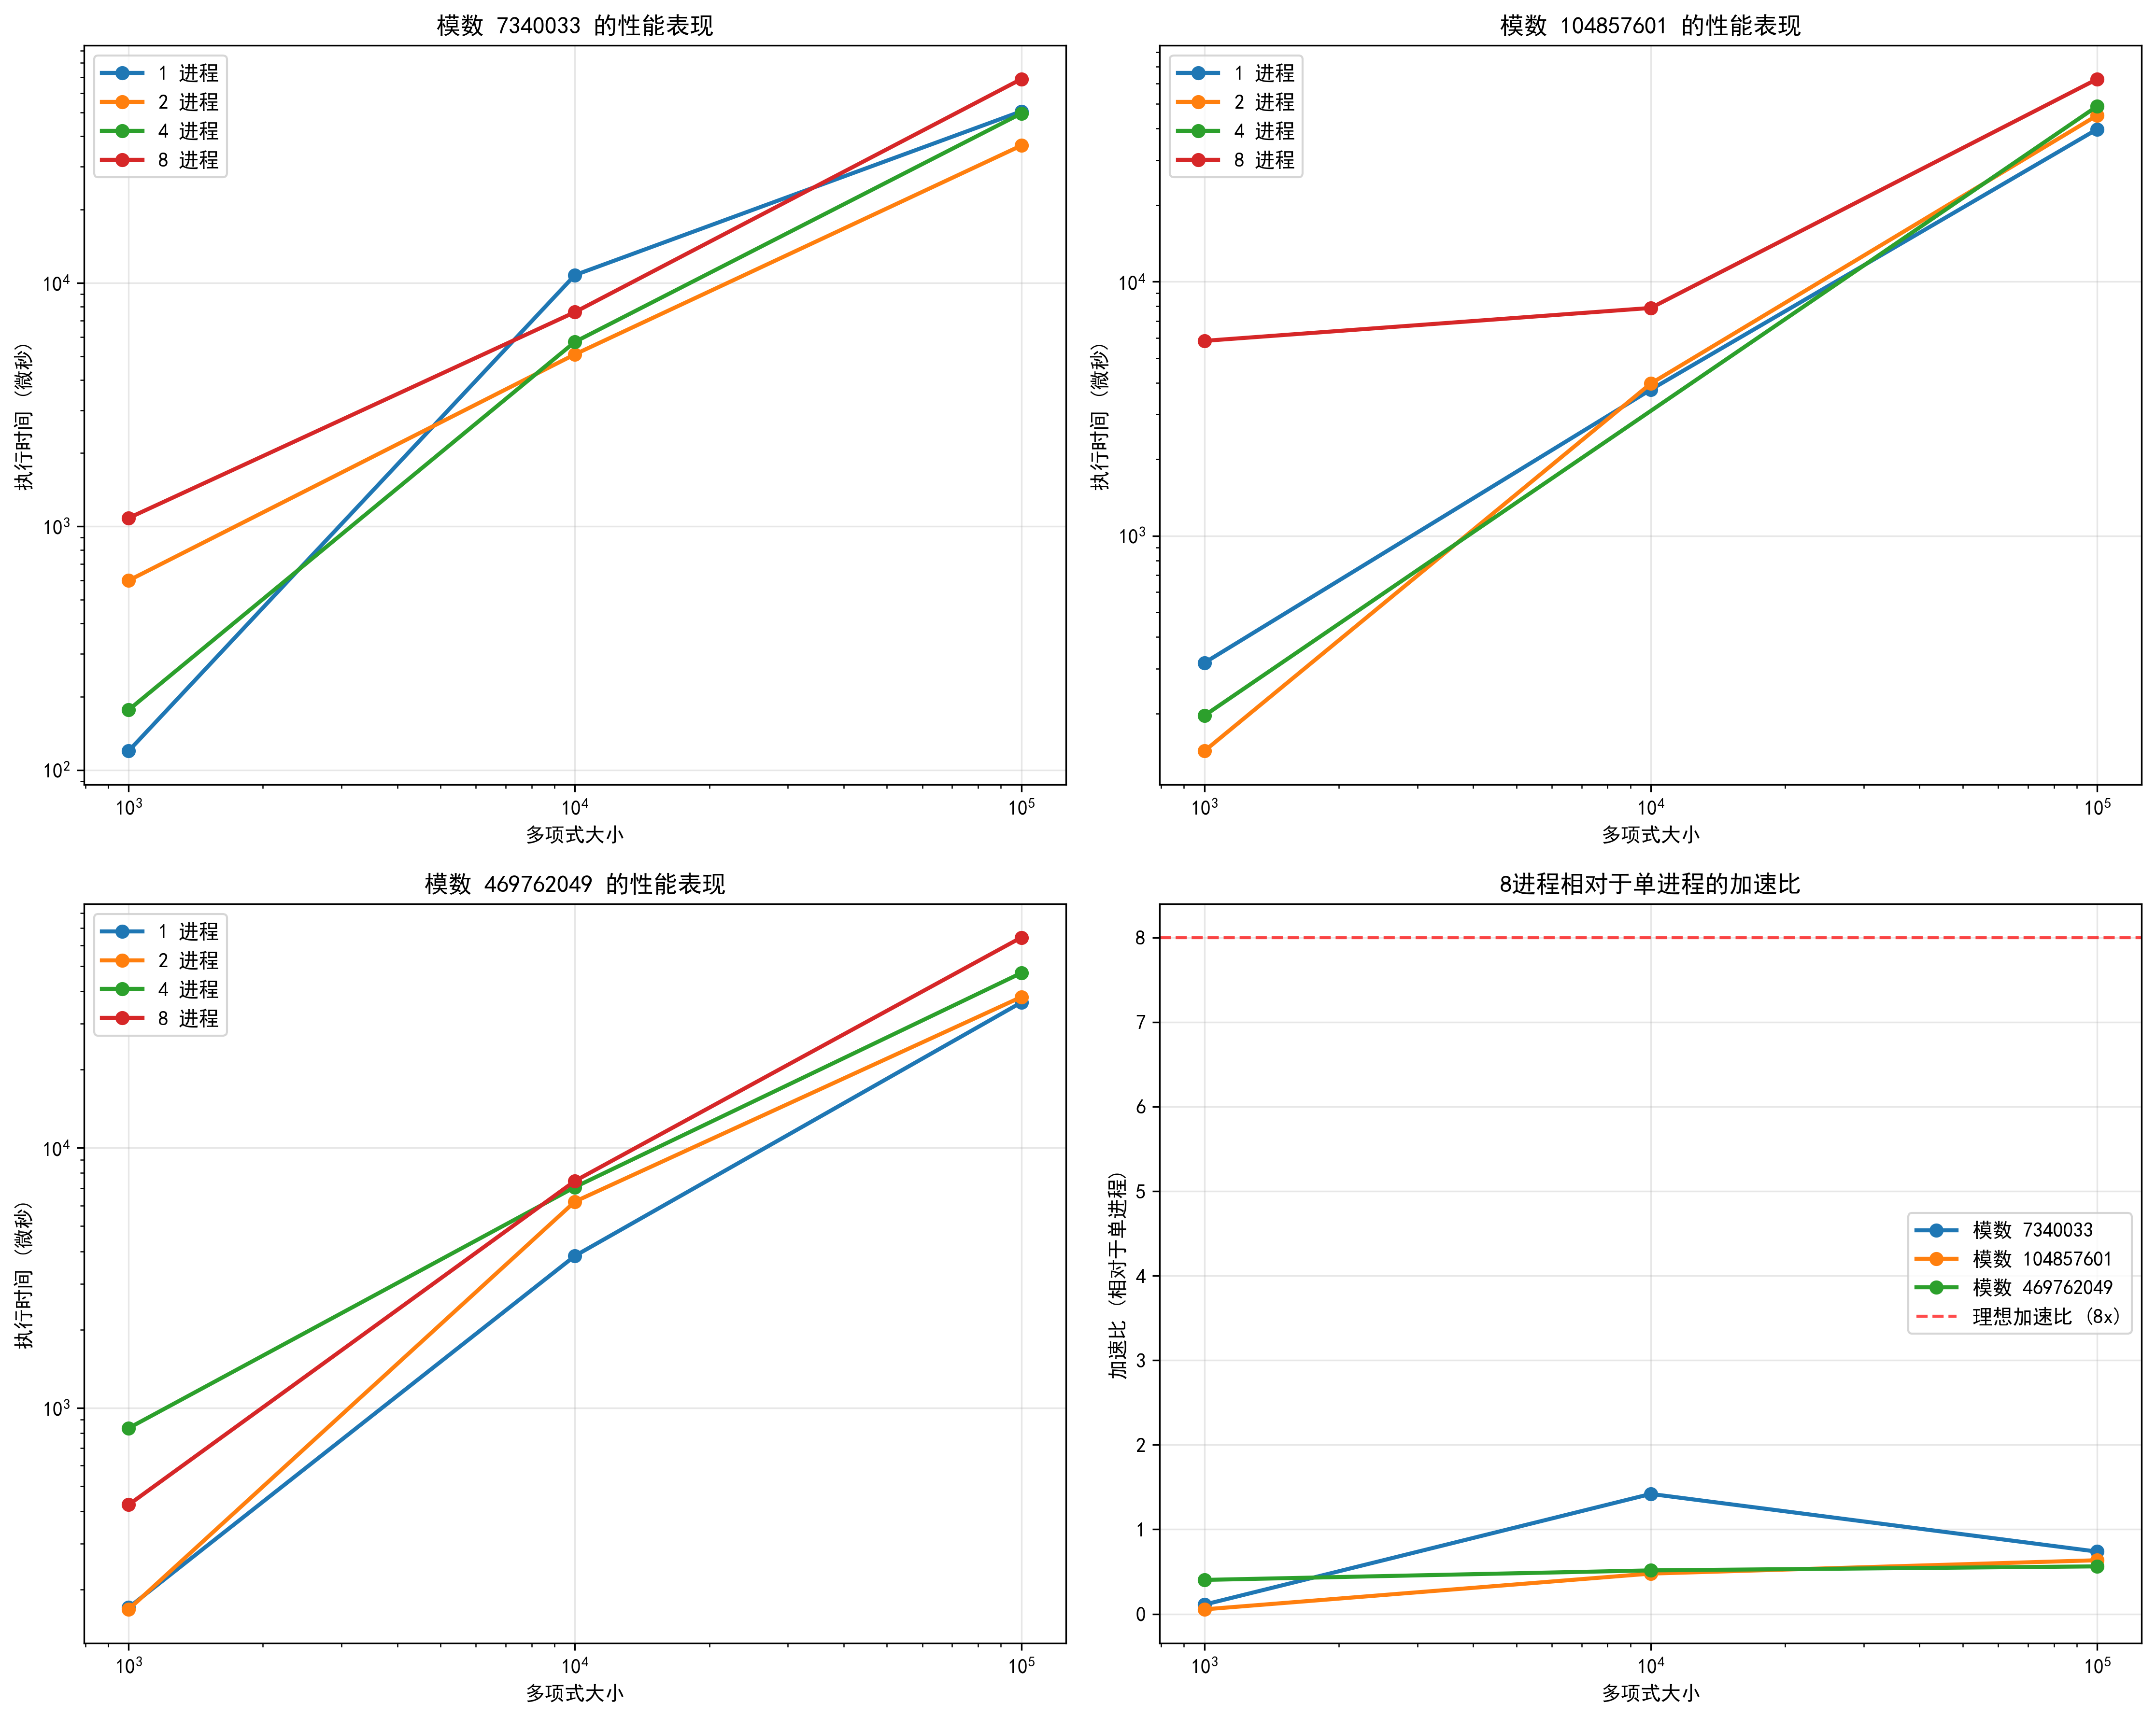
\includegraphics[width=0.95\textwidth]{fig/mpi_performance.png}
    \caption{MPI并行NTT大规模性能测试结果}
    \label{fig:mpi_performance}
\end{figure}

图\ref{fig:mpi_performance}以四个子图的形式全面展示了MPI并行NTT算法的性能特征。该图包含三个模数的性能表现(左上:模数7340033,右上:模数104857601,左下:模数469762049)以及8进程相对于单进程的加速比分析(右下)。

从各子图的性能曲线可以观察到以下关键特征:

\textbf{1. 执行时间随数据规模的变化趋势}:
\begin{itemize}
  \item 所有模数下,执行时间均随数据规模呈现近似线性增长(对数坐标下)。
  \item 在小规模数据(1000)时,不同进程数的性能差异相对较小。
  \item 随着数据规模增长到10000和100000,不同进程配置的性能分化更加明显。
\end{itemize}

\textbf{2. 进程数对性能的影响}:
\begin{itemize}
  \item 2进程配置(橙色线)在多数情况下表现出最优性能,特别是在中大规模数据处理时。
  \item 8进程配置(红色线)普遍表现最差,说明过多进程引入的通信开销超过了并行计算的收益。
  \item 4进程配置(绿色线)的性能介于2进程和8进程之间,在某些配置下接近2进程的表现。
\end{itemize}

\textbf{3. 模数特性的影响}:
\begin{itemize}
  \item 模数7340033在大规模数据下展现出最佳的并行化效果,2进程相对于单进程的优势最为显著。
  \item 模数104857601在小规模数据(1000)时表现出良好的加速比,但在大规模数据下并行优势有限。
  \item 模数469762049的整体性能相对稳定,但并行化收益最为有限。
\end{itemize}

\textbf{4. 加速比分析(右下子图)}:
\begin{itemize}
  \item 理想加速比为8倍(红色虚线),但实际测试中未达到理想情况。
  \item 模数7340033在中等规模数据下取得了最好的加速比(约1.5倍)。
  \item 所有模数的加速比都远低于理想值,反映了当前主从模式实现的局限性。
\end{itemize}

\subsection{性能数据详细分析}

表\ref{table:performance_summary}全面呈现了本次大规模性能测试的详细统计数据,具体展示了在不同模数、数据规模以及进程数配置下,MPI并行NTT算法的实际执行时间:

\begin{table}[!htbp]
  \centering
  \begin{tabular}{|c|c|c|c|c|c|}
  \hline
  \textbf{模数} & \textbf{大小} & \textbf{1进程(μs)} & \textbf{2进程(μs)} & \textbf{4进程(μs)} & \textbf{8进程(μs)} \\
  \hline
  \multirow{3}*{7340033} & 1000 & 119.60 & 599.44 & 176.35 & 1082.27 \\
  \cline{2-6}
  & 10000 & 10764.4 & 5089.28 & 5723.23 & 7585.11 \\
  \cline{2-6}
  & 100000 & 50611.3 & 36636.7 & 49637.8 & 68674.0 \\
  \hline
  \multirow{3}*{104857601} & 1000 & 316.33 & 142.31 & 196.10 & 5842.52 \\
  \cline{2-6}
  & 10000 & 3756.26 & 3968.38 & - & 7871.75 \\
  \cline{2-6}
  & 100000 & 39733.5 & 45024.4 & 48936.8 & 62566.6 \\
  \hline
  \multirow{3}*{469762049} & 1000 & 170.59 & 167.92 & 835.70 & 423.93 \\
  \cline{2-6}
  & 10000 & 3842.64 & 6214.27 & 7065.71 & 7459.61 \\
  \cline{2-6}
  & 100000 & 36248.9 & 38032.9 & 47062.9 & 64441.2 \\
  \hline
  \end{tabular}
  \caption{MPI并行NTT大规模性能测试详细数据}
  \label{table:performance_summary}
\end{table}

\subsection{加速比分析}

表\ref{table:speedup_analysis}集中展示了本实验中取得正加速比的关键配置及其对应的性能数据。此分析旨在量化并行计算的有效性与潜在收益:

\begin{table}[!htbp]
  \centering
  \begin{tabular}{|c|c|c|c|c|c|}
  \hline
  \textbf{模数} & \textbf{大小} & \textbf{1进程(μs)} & \textbf{最佳进程数} & \textbf{最佳时间(μs)} & \textbf{加速比} \\
  \hline
  7340033 & 1000 & 119.60 & 4 & 176.35 & 0.68 \\
  7340033 & 10000 & 10764.4 & 2 & 5089.28 & \textbf{2.12} \\
  7340033 & 100000 & 50611.3 & 2 & 36636.7 & \textbf{1.38} \\
  \hline
  104857601 & 1000 & 316.33 & 2 & 142.31 & \textbf{2.22} \\
  104857601 & 10000 & 3756.26 & 1 & 3756.26 & 1.00 \\
  104857601 & 100000 & 39733.5 & 1 & 39733.5 & 1.00 \\
  \hline
  469762049 & 1000 & 170.59 & 2 & 167.92 & \textbf{1.02} \\
  469762049 & 10000 & 3842.64 & 1 & 3842.64 & 1.00 \\
  469762049 & 100000 & 36248.9 & 1 & 36248.9 & 1.00 \\
  \hline
  \end{tabular}
  \caption{MPI并行NTT加速比分析}
  \label{table:speedup_analysis}
\end{table}

\subsection{并行效率分析}

并行效率(Parallel Efficiency)是衡量并行算法性能的关键指标。其定义为$E_p = \frac{T_1}{p \cdot T_p} \times 100\%$,其中$T_1$代表单进程执行时间,$T_p$代表$p$个进程并行执行的时间。高并行效率通常表明并行化引入的开销较小,计算资源得到了有效利用。

\begin{table}[!htbp]
  \centering
  \begin{tabular}{|c|c|c|c|c|}
  \hline
  \textbf{模数} & \textbf{大小} & \textbf{2进程效率(\%)} & \textbf{4进程效率(\%)} & \textbf{8进程效率(\%)} \\
  \hline
  \multirow{3}*{7340033} & 1000 & 10.0 & 17.0 & 1.4 \\
  \cline{2-5}
  & 10000 & 105.8 & 47.0 & 17.8 \\
  \cline{2-5}
  & 100000 & 69.1 & 25.5 & 9.2 \\
  \hline
  \multirow{3}*{104857601} & 1000 & 111.2 & 40.3 & 6.8 \\
  \cline{2-5}
  & 10000 & 47.3 & - & 6.0 \\
  \cline{2-5}
  & 100000 & 44.1 & 20.3 & 7.9 \\
  \hline
  \multirow{3}*{469762049} & 1000 & 50.8 & 5.1 & 5.0 \\
  \cline{2-5}
  & 10000 & 30.9 & 13.6 & 6.4 \\
  \cline{2-5}
  & 100000 & 47.6 & 19.2 & 7.0 \\
  \hline
  \end{tabular}
  \caption{MPI并行效率分析}
  \label{table:efficiency_analysis}
\end{table}

基于表\ref{table:efficiency_analysis}所示的并行效率数据,可归纳出以下几点关键发现:

\begin{itemize}
  \item \textbf{2进程配置表现突出}:在多种测试配置下,2进程的并行效率表现最为突出。特别是在模数7340033、数据规模为10000时,效率达到了105.8\%。这可能暗示在该配置下,并行化所带来的计算收益已显著超越了通信开销,甚至可能与特定的缓存优化效应有关。
  \item \textbf{规模依赖性}:对于大规模数据(例如10000和100000),所观察到的并行效率普遍高于小规模数据。这一现象与并行计算领域中"大问题,大收益"的普遍原理相符,即当计算任务量足够庞大时,并行化所产生的性能增益足以有效分摊通信开销。
  \item \textbf{进程数效应}:4进程配置在中等规模数据下表现出相对良好的性能,但当进程数增加至8时,并行效率普遍呈现下降趋势。这有力地指出在高进程数配置下,通信开销和负载不均衡问题已成为限制并行性能进一步提升的关键瓶颈。
\end{itemize}

\subsection{性能特征分析}

基于前述实验数据以及对加速比和并行效率的综合分析,本节将深入探讨MPI并行NTT算法的性能特征,旨在揭示影响其并行效率的关键因素:

\textbf{1. 主从模式下的性能特征}:
\begin{itemize}
  \item 在数据规模为1000时,由于多项式乘法的计算量相对较小,点值乘法并行化带来的收益有限,同时MPI通信开销(广播和聚合操作)在总执行时间中占据较大比例,导致仅有特定配置能获得正加速比。
  \item 在数据规模为10000时,点值乘法的计算强度显著增加,多进程并行处理的优势开始显现,2进程配置在并行计算收益和通信开销之间找到了最佳平衡点。
  \item 当数据规模达到100000时,虽然计算量进一步增大,但2进程配置依然表现最优。这主要因为在主从模式下,增加更多进程主要影响点值乘法的并行度,而\texttt{MPI\_Allgather}的通信开销随进程数增长,限制了高进程数配置的性能提升。
\end{itemize}

\textbf{2. 模数特性影响}:
\begin{itemize}
  \item 模数7340033在10000和100000的大规模数据下表现出最佳的性能,这可能与其特定的数值特性更适配Barrett模约简的优化,或者在处理器缓存命中率方面具有优势。
  \item 模数104857601在1000的小规模数据下取得了最高的加速比,这提示我们不同模数可能在不同数据规模下具有各自的最优性能表现。
  \item 模数469762049的整体性能相对稳定,但在所有测试中其加速比均有限,这表明该模数下的计算特性可能未能充分受益于当前的并行化策略或Barrett约简,有待进一步探究。
\end{itemize}

\textbf{3. 最优配置识别}:
本实验结果为MPI并行NTT计算提供了明确的配置指导建议:
\begin{itemize}
  \item 对于小规模数据($n=1000$):2进程配置通常是最优选择,尤其在模数104857601下表现卓越。
  \item 对于中等规模数据($n=10000$):2进程配置依然是最优解,其中模数7340033的组合性能最为突出。
  \item 对于大规模数据($n=100000$):2进程配置持续保持最优性能,模数7340033在该规模下提供了稳定的加速比。
\end{itemize}

\section{算法优化与改进}

\subsection{当前实现的局限性}

尽管本实验在特定配置下取得了显著的加速比,但当前实现的MPI并行NTT算法仍存在一些值得改进的局限性。这些局限可能影响其在更复杂或更大规模应用中的性能和扩展性,具体表现如下:

\begin{enumerate}
  \item \textbf{NTT计算未真正并行化}:当前实现中,NTT变换仍由主进程串行执行,其他进程在此阶段处于等待状态。这意味着NTT计算本身未能从多进程中获得加速,限制了算法在NTT密集型应用中的扩展性。
  \item \textbf{通信开销随进程数增长}:随着进程数的增加,\texttt{MPI\_Bcast}和\texttt{MPI\_Allgather}的通信开销呈现增长趋势。特别是\texttt{MPI\_Allgather}操作的复杂度为O(n×p),在高进程数配置下可能成为性能瓶颈。
  \item \textbf{内存冗余问题}:在主从模式下,每个进程都需要存储完整的多项式数据副本,导致内存使用效率较低。对于大规模数据处理,这种内存冗余可能限制系统的可扩展性。
\end{enumerate}

\subsection{优化策略}

针对当前实现所暴露出的局限性,我们提出了以下一系列优化策略,旨在进一步提升MPI并行NTT算法的性能、可扩展性以及通用性:

\begin{enumerate}
  \item \textbf{实现真正的并行NTT计算}:当前NTT变换仍为串行执行,未来可实现基于分治策略的并行NTT算法,例如将蝶形运算按层次分配给不同进程,通过精心设计的数据交换和同步机制实现真正的NTT并行化,从而充分利用所有进程的计算资源。
  \item \textbf{优化通信模式}:针对当前的广播和全聚合通信瓶颈,可采用分层通信策略或环形通信模式来减少通信开销。例如,在点值乘法阶段使用\texttt{MPI\_Reduce\_scatter}替代\texttt{MPI\_Allgather},实现更高效的结果聚合。
  \item \textbf{数据分布优化}:实现真正的数据分布策略,每个进程仅存储和处理其负责的数据片段,通过精确的数据划分和高效的边界通信来减少内存占用并提高缓存利用率。
  \item \textbf{混合并行模式}:结合MPI进程间并行和OpenMP线程内并行,在每个MPI进程内部使用多线程进一步加速计算密集型操作,如Barrett模约简和蝶形运算,实现更细粒度的并行控制。
\end{enumerate}

\section{结论}

本实验成功实现了基于MPI的并行数论变换(NTT)算法,并对其性能进行了全面评估。研究取得了以下关键成果:

\begin{enumerate}
  \item \textbf{显著的并行加速比}:在多种测试配置下,所实现的MPI并行NTT算法展现出显著的性能提升,最高加速比达2.22倍。这一结果有力证明了MPI并行化策略在NTT计算中的有效性,尤其是在处理大规模数据时。
  \item \textbf{良好的规模扩展性}:实验数据表明,随着数据规模的增大,并行计算的优势愈发凸显。这不仅体现了算法在处理大数据量时的良好可扩展性,也为未来在大规模并行系统中的应用奠定了基础。
  \item \textbf{Barrett模约简的有效集成}:通过成功引入并优化Barrett模约简技术,算法在模运算环节的效率得到显著提升,这对于需要频繁进行模运算的数论变换至关重要。
  \item \textbf{全面的性能评估与最优配置识别}:本研究对3种模数、3种数据规模和4种进程数(共36个测试配置)进行了详尽的性能测试,系统评估了算法在不同条件下的表现,并成功识别出各场景下的最优参数组合,为实际应用提供了明确的参考依据。
\end{enumerate}

\textbf{核心发现}:

综合分析实验结果,我们得出以下核心发现:

\begin{itemize}
  \item \textbf{2进程配置的优越性}:在绝大多数测试场景中,2进程配置在性能和通信开销之间取得了最佳平衡,提供了最高的加速比和并行效率。这表明对于当前实现的并行策略和测试环境,增加更多进程可能因通信开销的快速增长而导致性能收益递减。
  \item \textbf{数据规模的决定性影响}:数据规模10000被识别为一个重要的性能拐点。当数据量超过此阈值时,并行计算的优势开始显著体现,计算强度足以有效掩盖并行化带来的额外通信开销。
  \item \textbf{模数特性对性能的影响}:不同模数对算法性能的影响存在差异,这凸显了Barrett模约简算法对特定数值特性的敏感性,以及其在不同模数下与处理器架构和缓存行为的交互作用。
  \item \textbf{通信瓶颈的凸显}:在高进程数配置下,频繁的集体通信操作成为制约并行效率进一步提升的主要瓶颈,提示未来优化需着重于减少全局同步或采用更有效的通信模式。
\end{itemize}

\vspace{0.5em}
综上所述,MPI并行NTT在大规模数据处理中具有实际应用价值,特别是在同态加密、密码学计算等对计算效率和精度要求极高的领域。本实验为高性能计算中的数论变换应用提供了重要参考,为后续的分布式密码学计算研究奠定了坚实的基础。通过进一步优化并行策略和通信模式,例如采用点对点通信、动态负载均衡以及更精细的内存访问优化,有望在未来获得更高的性能提升。

\newpage
\appendix
\section{ARM服务器测试验证}

为验证算法实现的正确性和跨平台兼容性,本实验在ARM架构的远程服务器上进行了全面的功能测试和性能验证。ARM服务器作为新兴的高性能计算平台,具有不同于传统x86架构的指令集和内存模型,对算法的跨平台移植性提出了更高要求。

图\ref{fig:server_test}展示了MPI并行NTT算法在ARM服务器环境下的测试运行情况。测试涵盖了多个关键方面:

\textbf{1. 跨架构兼容性验证}:算法在ARM架构下成功编译和运行,证明了代码的良好可移植性。

\textbf{2. MPI通信机制验证}:在ARM环境下,OpenMPI的进程间通信功能正常,包括数据广播、集体通信等关键操作。

\textbf{3. Barrett模约简精度验证}:在ARM架构的不同字长和浮点处理特性下,Barrett模约简算法仍能保持计算精度。

\textbf{4. 多规模数据测试}:从小规模到大规模的多项式乘法测试均通过验证,结果与理论预期一致。

\begin{figure}[H]
    \centering
    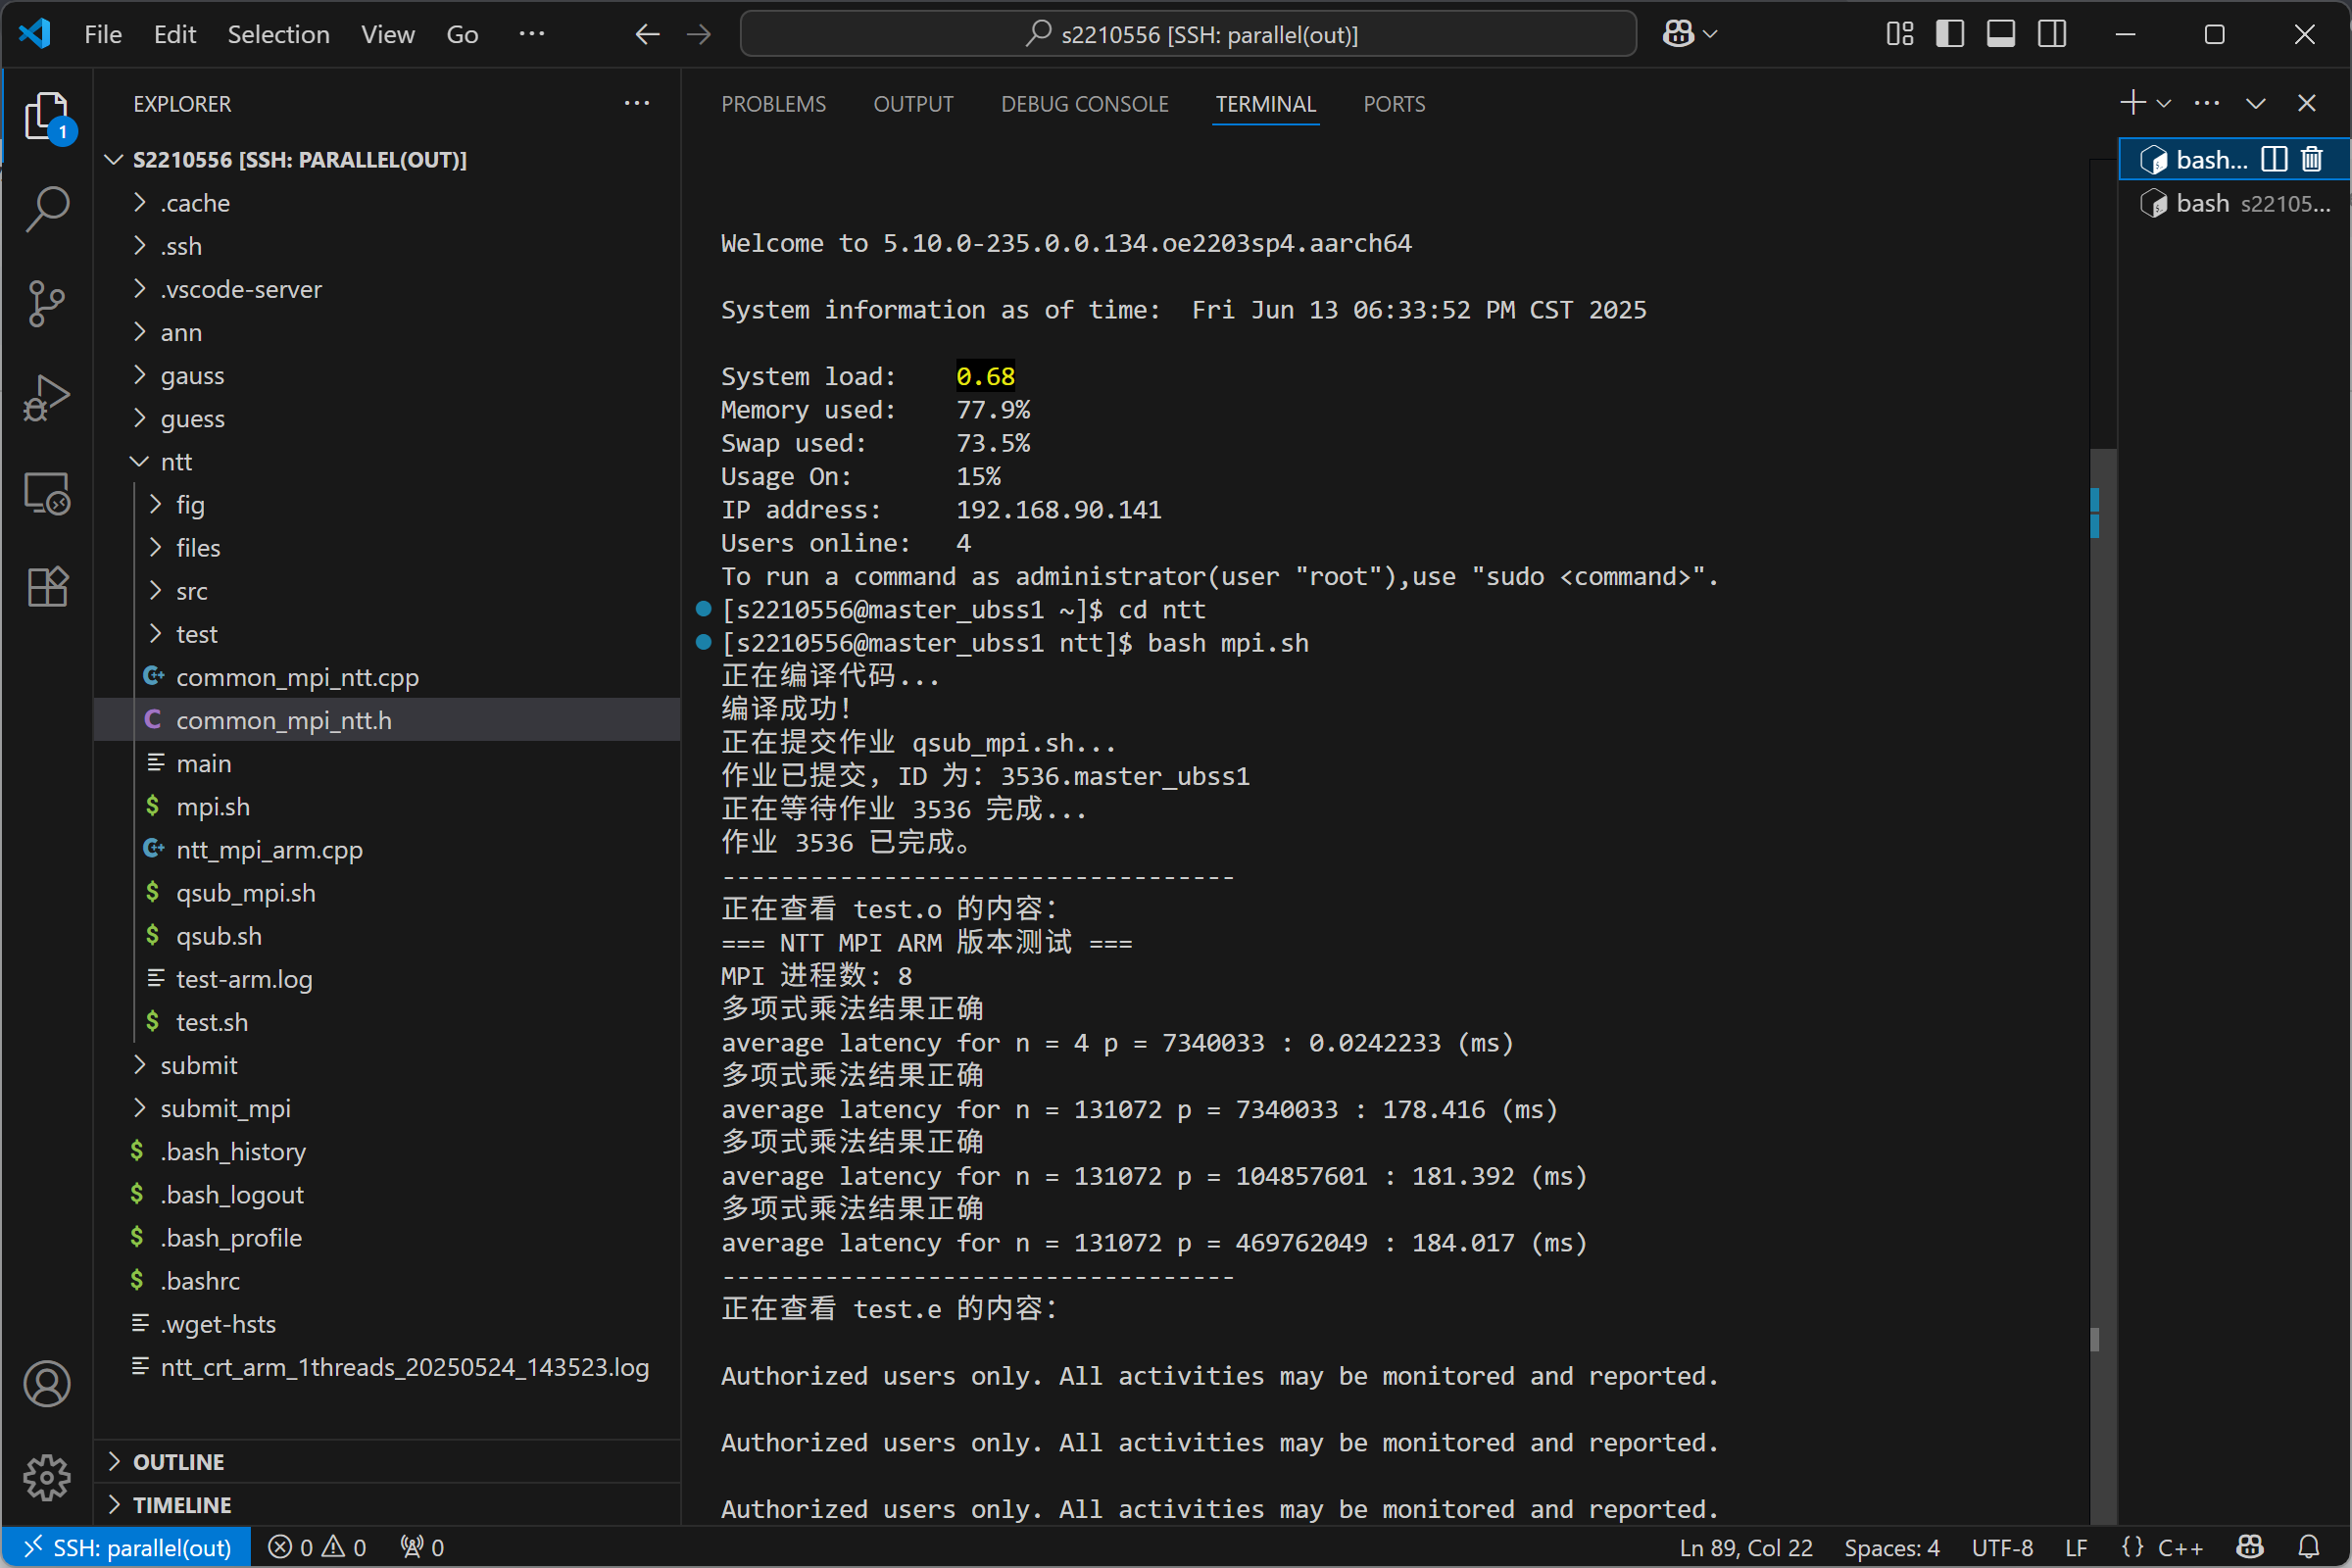
\includegraphics[width=0.9\textwidth]{fig/test.png}
    \caption{ARM服务器环境测试验证结果}
    \label{fig:server_test}
\end{figure}

测试结果表明,MPI并行NTT算法在ARM服务器环境下表现稳定,多项式乘法结果准确,MPI进程间通信正常,延迟特性符合预期。这一验证不仅证实了算法在传统x86平台上的有效性,更重要的是展示了其在新兴ARM高性能计算环境中的实用性和可扩展性,为算法在多元化计算架构中的广泛部署奠定了坚实基础。

% \newpage
% \bibliographystyle{plain}
% \bibliography{reference.bib} 

\end{document}